\documentclass[12pt, a4paper]{report}

%==============================================================================
% PACKAGES
%==============================================================================
\usepackage[utf8]{inputenc} % For text encoding
\usepackage{xcolor}         % For defining custom colors
\usepackage{tocloft} 
\usepackage{amsmath}        % For math equations
\usepackage{hyperref}       % For clickable links in the PDF
\usepackage[margin=1in]{geometry}
\usepackage{setspace}
\usepackage{lmodern}
\usepackage[T1]{fontenc}
\usepackage[protrusion=true,expansion=true]{microtype} % load after lmodern
\usepackage{graphicx}
\usepackage{enumitem}
\usepackage{titlesec}
\usepackage{ragged2e}
\usepackage{parskip} % no paragraph indent, adds space
\usepackage{caption}
\usepackage{fancyhdr}
\usepackage{amssymb} % For \checkmark symbol
\usepackage{enumitem}

\usepackage{listings} % for code

% Code styling
\lstset{
    language=C,                         % Set language (C for DNS code)
    basicstyle=\ttfamily\footnotesize,  % Font style
    numbers=left,                       % Line numbers on the left
    numberstyle=\tiny\color{gray},      % Style for line numbers
    keywordstyle=\color{blue},          % Keywords in blue
    commentstyle=\color{green!50!black},% Comments in green
    stringstyle=\color{orange},         % Strings in orange
    frame=single,                       % Border around code
    breaklines=true,                    % Wrap long lines
    captionpos=b,                       % Caption at the bottom
    tabsize=4,                          % Tab = 4 spaces
    showstringspaces=false              % Don’t show spaces in strings
}

%==============================================================================
% DOCUMENT SETUP
%==============================================================================

% Set page margins
\geometry{a4paper, margin=1in}

% Define the custom orange color from your title page image
\definecolor{customOrange}{HTML}{D28A32}
\definecolor{sectionbar}{HTML}{E9A640} % orange bar color similar to the image
\definecolor{sectiontext}{HTML}{2B2B2B}

% Setup for hyperref (makes ToC and references clickable)
\hypersetup{
    colorlinks=true,
    linkcolor=black,
    urlcolor=blue,
    citecolor=black
}

% Wide, colored bar style for "section-like" headers
\newcommand{\sectionbar}[1]{%
  \vspace{0.6\baselineskip}%
  \noindent
  \colorbox{sectionbar}{%
    \parbox{\dimexpr\linewidth-2\fboxsep\relax}{%
      \textbf{\Large\textsf{#1}}%
    }%
  }%
  \vspace{0.6\baselineskip}
}

% Body text tweaks
\setstretch{1.2}
\setlist[itemize]{leftmargin=1.2em}
\setlist[enumerate]{leftmargin=1.2em}

% Section title spacing (not used directly since we use custom bars)
\titlespacing*{\section}{0pt}{1ex}{0.6ex}

% Figure captions smaller and tight
\captionsetup{font=small,labelfont=bf}

% Footer with page number
\pagestyle{fancy}
\fancyhf{}
\cfoot{\thepage}

%==============================================================================
% BEGIN DOCUMENT
%==============================================================================
\begin{document}

%==============================================================================
% TITLE PAGE
% This is a custom title page environment to replicate your image.
%==============================================================================
\begin{titlepage}
    \centering
    \vspace*{\fill} % Pushes content down vertically
    
    % --- Main Title ---
    {\Huge\bfseries ASSIGNMENT 1}
    
    \vspace{0.75cm} % Space between title and subtitle
    
    % --- Subtitle ---
    {\Large\bfseries Computer Networks}
    
    \vfill % Flexible vertical space
    
    % --- Author Info Box ---
    % \colorbox creates the colored background
    % \parbox creates a container for the text inside
    \colorbox{customOrange}{%
        \parbox{1.0\textwidth}{%
            \centering
            \vspace{1em} % Padding top
            {\Large\color{white} Tejas Lohia, Umang Shikarvar} \\[0.5em] % Your name
            {\large\color{white} 23110335, 23110301} % Your ID
            \vspace{1em} % Padding bottom
        }
    }
    
    \vspace*{\fill} % Pushes the author box up from the bottom
\end{titlepage}


%==============================================================================
% FRONT MATTER (Table of Contents, etc.)
%==============================================================================
% \pagenumbering{arabic}


\renewcommand{\cfttoctitlefont}{\hfill} 
\renewcommand{\cftaftertoctitle}{\hfill}
{\noindent{\parbox{\textwidth}{\vspace{0.4em}\Large\bfseries\color{white}\hspace{1em}TABLE OF CONTENTS\vspace{0.4em}}}}

% --- Generate the list of contents ---
\tableofcontents 

%=================================
%       LABORATORY SESSION 1
%=================================
\chapter{DNS Resolver}
\section{Introduction}

\subsection{DNS:}

The domain server name is one of the most critical protocols in computer Networks. It is highly preferrable for a user to input human-friendly domain names such as www.google.com. However, to make these interpretable to the networking protcols to avail services, a system is required which would convert human-friendly domain names to machine-level IP Addresses. DNS acts as a distributed and heirarchical translator, making them very fundamental in the computer networks as it would be very difficult for users to remember numerical IP Addresses. DNS provides a seamless service to the clients to get the IP Addresses using a heirarchical server presence. Citing the central role, DNS is an important subject of study in research in computer networks.


\subsection{PCAP files:}

PCAP files are critical in the practical network analysis. These files contain packet datas that have been captured from interfaces of live networks using tools like tcpdump and wireshark. PCAP files store packet data in sequential order which allows users to study and dissect network traffic post capture, without relying on the active network connection. This provides an environment to study real time packets instead of working with artificially generated packets.

\subsection{DNS resolver:}

DNS resolver is a network service responsible for the tranlation by acting as an intermediary between client such as web browser and DNS system. When there is a DNS query, it is handled and resolved either by returning the cache if exists or by requesting from the DNS servers.

\
\section{Tools}

\begin{itemize}
    \item \textbf{Programming Language:} C language and Python 3.12.9
    \item \textbf{Editor/IDE:} Visual Studio Code --- Used for coding, debugging and execution.
    \item \textbf{Version Control:} Git and GitHub --- Used to track and the changes in the code, and to improve maintainability of the codebases.
    \item \textbf{Virtual Environment:} assign1 --- To prevent library version conflicts by isolating working environments.
    \item \textbf{wireshark:} --- To verify the results obtained by the codes over PCAP files.
\end{itemize}

\
\section{Methodology and System Design}


The overall workflow adopted for this project was to analyze the DNS data from packet capture files. The file contained data for multiple protocols, out of which only entries corresponding for DNS queries were extracted.
The client file reads packets from .pcap file, parses them to extract the DNS data from thses packets. The data is concatenated with custom data of 8 bytes containing information about custom header containing time and sequence\_id and is passed to the server. The server in turn returns the domain name from the DNS data passed to it.

Code is written at a low level without actually using the pcap library. Code parses each of the packet, filters based on the type and then slices the network layer packets to obtain the raw data.

At high level the code follows the conventional client-server model. Client sends the DNS queries and server returns the IP address over UDP protocol which is preferrably used for DNS protocol.


\newpage
\subsection{Main () function of client}

\begin{lstlisting}[caption={Opening the files}]
int main(int argc, char *argv[]) {
    
   // if (argc != 2) {
   //     printf("Usage: %s <pcap file>\n", argv[0]);
   //     return 1;
   // }

    printf("PCAP Client\n");
    //char *filename = argv[1];
    //char *filename = "./p.pcap";

    // Set the pcap file to be processed
    char *filename = "./6.pcap"; 
    
    //file which would be used to anayze the DNS packets
    char *dnsFileName="./dns.txt";

    dnsFile = fopen(dnsFileName, "w");
    
    dnsReportFp = fopen("./dnsReport.txt", "w");

    
    if (!dnsReportFp) {
        printf("Failed to open file\n");
        return -1;
    }

/*
    Opening the pcap file in the binary format which is stored in the little Endian format in the memory.
*/
    FILE *fp = fopen(filename, "rb");

    if (!fp) {
        printf("Failed to open file\n");
        return -1;
    }

\end{lstlisting}

\textbf{Opening files}

This part of the code opens 6pcap files in binary format as \textbf{fp} which is stored in binary format in Little Endian.
dnsReport file is opened to store the required content which stores CustomHeaderFile, Domainname and resolved IP Addresses.
Another file dns.txt is opened to store the DNS data extracted from the packets to debug.

\newpage


\begin{lstlisting}[caption={Creating the socket and checking the validity of the pcap file}]

    create_dns_client_socket(); //we initialize the client socket and configures the server_address 

    pcap_hdr_t header; //will store the header of the pcap file

/*
pcap file opened in binary format
fread : C library call to read the binary data.
It copies the first sizeof(header) amount of content to the structure.
This structure is the header of the pcap file
*/

    size_t read_bytes = fread(&header, 1, sizeof(header), fp);
    if (read_bytes != sizeof(header)) {
        printf("Failed to read pcap header\n");
        fclose(fp);
        return -1;
    }

    //printing the header of the pcap file
    print_global_header(&header);

/*

Magic number is used to validate the type of the file.
Magic number : 0xa1b2c3d4 confirms pcap file
*/    

    if(header.magic_number != 0xa1b2c3d4){
        printf("%s is not valid pcap file\n",argv[1]);
        exit(-1);
    }

\end{lstlisting}

\textbf{Socket Initialization}

This part of the code calls the create\_dns\_client\_socket function which creates the socket for client and initializes server address.
A structure is initialized of the type pcap. header, which is used to copy the pcap header data from the pcap file. Pointer to this structure is passed to a library system call fread to obtain the data, which equals the size of the of the structure.
Another function print\_global\_header is called to print the header information extracted from the pcap file while incrementing the file read pointer.

\textbf{Magic Number: } They are used to check the type of the opened file.
xa1b2c3d4 is the magic number for the pcap filetype. Code exists in case the magic number obtained does not match the xa1b2c3d4, as it indicates improper file type.


\begin{lstlisting}[caption={Iterating over the pcap file}]

fprintf(dnsReportFp,"\tCustomHeaderFile\tDomainname\t\tResolved IP Address\n");
    fprintf(dnsReportFp,"\t  (HHMMSSID)\n\n");
    
    while(len > 0){
        record_packet1=NULL;
        printf("packet no %d\n",record_num++);

/*

read_pcap_packet is called, which fetches the length of the packet.
Importantly it also allocates memory to the packet read and record_packet1 points to the array where packet is stored.

*/

        len=read_pcap_packet(fp,&record_packet1);


        if(len == 0 ){
            printf("end of file\n"); //len 
            break;
        }

        if(len == -1){
            printf("Error in the reading the packet\n");
            printf("Breaking the loop\n");
            break;
        }

        //printf("address %p",(void *)record_packet1);
        //printf("Packet data (first 32 bytes or less):\n");
        //for (uint32_t i = 0; i < 32; i++) {
        //      printf("%02x ", *(record_packet1+i));
        //}
        //printf("\n");
        //ethernet_header_t *eth=(ethernet_header_t *)record_packet1;
        //printf("ethernet type %x\n",eth->ethertype);
        //if (ntohs(eth->ethertype) != 0x0800) {
        //    printf("Not an IPv4 packet\n\n");
        //    return (-1);
        //}

        //getting the offset in the packet to point at the DNS data

        dns_offset=parse_pcap_packet(record_packet1,len);
        dns_packet_size=len-dns_offset;
        dns_custom_packet_size= dns_packet_size+8;


\end{lstlisting}

\textbf{Iteration over all the packets}

This part of the code iterates through all the packets in the pcap file. 

record\_packet1 is a pointer to an array of characters which will point to the array storing the each packet data.

Function read\_pcap\_packet function is called with over the pointer to the current packet in the file and the pointer to store the data.

if the function returns 0, code exits as it has reached the end of the pcap file, else if the function returns -1, then there was some error in reading packet and the loop breaks.

From the array containing the packet data, to extract the DNS data we are required to find the offset to reach the DNS data. 

Function parse\_pcap\_packet is invoked to find the offset in that array.

As the custom added header would be of 8 bytes, the size of the final packet would be \textbf{length of the original packet - dns offset} which gives the length of the DNS data + 8, which is the size of the custom header added.

\vspace{3em} 

\begin{lstlisting}[caption={Processing the DNS packet, DNS querying and storing the results}]

if(dns_offset > 0) // Meaning DNS packet
        {
            //printf("DNS packet\n");
            //fprintf(dnsFile,"DNS offset %d %d\n",dns_offset,len);
            //for(int i=0;i< (dns_packet_size);i++)
            //    fprintf(dnsFile,"%02x ", *(record_packet1+i+dns_offset));

            //dns_name extracts the human readable domain name by accessing the DNS data in the packet.
            dns_name((record_packet1+dns_offset+12),dn_query_name);
            

            fprintf(dnsFile,"\n Total Bytes %d : %s",dns_custom_packet_size,dn_query_name);

            //custom_dns_packet structure stores the final packet containing the custom data header along with the DNS data.
            make_custom_packet(&custom_dns_packet,(record_packet1+dns_offset),dns_packet_size);

            // custom_dns_packet is sent to the server to get the ipv4 address.
            int bytesSent=send_dns_msg_to_server(custom_dns_packet,dns_custom_packet_size);
            fprintf(dnsFile,"\n  Bytes Sent %d : ",bytesSent);
            for(int i=0;i< (dns_packet_size+8);i++)
                fprintf(dnsFile,"%02x ", *(custom_dns_packet+i));
            //free(custom_dns_packet);
            //usleep(100000);

            //dns_reply_ip is contains the received IP address from the server.
            receive_dns_msg_from_server(dns_reply_ip,10);

            // custom_dns_packet is type casted to the structure storing the custom header data.
            dns_custom_header_t *dns_ch=(dns_custom_header_t*)(custom_dns_packet);

            //final data is stored to the dnsReport
            fprintf(dnsReportFp,"\t%02d%02d%02d%02d\t\t%s\t\t%s\n",
                            (int)dns_ch->hour,
                            (int)dns_ch->min,
                            (int)dns_ch->sec,
                            (int)dns_ch->seq_no,
                            dn_query_name,
                            dns_reply_ip

                            );
            free(custom_dns_packet);                
        }
        //printf("packet no %d\n",record_num++);
        if(record_packet1 != NULL)
            free(record_packet1);
    }

\end{lstlisting}

\textbf{Custom header addition, querying and receiving IPv4 address}

This is the critical part of the code which extracts the name from the packet data, queries to the DNS server and stores the received IPv4 address into the dnsReport file.

dns\_name function is invoked which passes the pointer to the final location where the DNS data starts in the record\_packet1 array and copies the human understandable name to the variable dn\_query\_name.

make\_custom\_packet function is called which combines the custom header data with the DNS data in the packet to store the final DNS query packet in variable custom\_dns\_packet. 

send\_dns\_msg\_to\_server function is invoked which finally sends the DNS query.

receive\_dns\_msg\_from\_server is invoked which receives the ip address reply from the server, and finally the data is stored in dnsReport.

\newpage
\subsection{Packet structures and global pointers}


\begin{lstlisting}[caption={socket, server\_addr and file pointers}]
int sockfd;
struct sockaddr_in server_addr;

FILE *dnsFile;
FILE *dnsReportFp;

\end{lstlisting}

socket stores the socket number.

server\_addr stores the information about the server IP, port and protocol over which the connection would be laid.

dnsFile and dnsReportFp are pointers to text files.
\vspace{1em}
\begin{lstlisting}[caption={Pcap file structure and pcap file header}]
/*
pcap file structure:
    24 bytes pcap header 
    16 bytes record header
    incl_len bytes record or packet (Can be for any type)
    (this repeats)
*/

// 24 Bytes for PCAP Header
typedef struct pcap_hdr_s {
    
    uint32_t magic_number;   /* magic number */
    uint16_t version_major;  /* major version number */
    uint16_t version_minor;  /* minor version number */
    uint32_t  thiszone;       /* GMT to local correction */
    uint32_t sigfigs;        /* accuracy of timestamps */
    uint32_t snaplen;        /* max length of captured packets, in octets */
    uint32_t network;        /* data link type */

} pcap_hdr_t;

\end{lstlisting}

\textbf{Understanding the pcap file stucture}

pcap file contains 24 bytes of header data. Next 16 bytes are the header for a packet, followed by packet with variable length. 

For every packet of variable length, there is a header of 16 bytes. So, there are alternating packet headers and packets.
\newpage
\textbf{Understanding the pcap header stucture}

Importantly pcap header file contains the magic number which is used to check whether the opened file is pcap file.
\newline 
This is followed by version umbers, offset to GMT, accuracy of the timestamps, max length of the captured packets and data link type.

\noindent\href{https://wiki.wireshark.org/Development/LibpcapFileFormat\#overview}{Ref: Libpcap File Format Overview (Wireshark Wiki)}

\vspace{1em}
\textbf{Packet headers}

\begin{lstlisting}[caption={Packet headers}]
/*
record header structure:
    This is a 16byte header before every record in the PCAP file.
    Third entry of this header gives information about the length of incl_len
    While forth entry gives the original length of the packet, in case cropped
*/

typedef struct pcaprec_hdr_s {
    uint32_t ts_sec;         /* timestamp seconds */
    uint32_t ts_usec;        /* timestamp microseconds */
    uint32_t incl_len;       /* number of octets of packet saved in file */
    uint32_t orig_len;       /* actual length of packet */
} pcaprec_hdr_t;
\end{lstlisting}

Two initial fields store the seconds and microseconds of the time packet received since the UNIX epoch.

Packets are of varied length, therefore incl\_len stores the length of the packet, while orig\_len stores the length of the original packet in cases where the packet has been sliced to some max length.

\noindent\href{https://wiki.wireshark.org/Development/LibpcapFileFormat\#overview}{Ref: Libpcap File Format Overview (Wireshark Wiki)}


\newpage
\vspace{1em}
\textbf{Packet Structures}

Record/Packet structure

    \begin{itemize}
        \item 14 bytes: Ethernet Header
        \item IPv4 Header (typically 20 bytes, but can be more with options)
        \item 8 bytes: UDP Header \textit{or} variable size for TCP Header / other protocol header
        \item 12 bytes: DNS Header \textit{or} other protocol header
        \item DNS Data / other data in packet
    \end{itemize}


Each of the packet contains a series of header data, and then the final data in the packet.

1. First header is the \textbf{Ethernet header} which is of 14 bytes containing 3 fields.

\textbf{Ethernet Structures}

\begin{lstlisting}[caption={Ethernet Header Structure}]
typedef struct ethernet_header_s{
    uint8_t dest_mac[6];
    uint8_t src_mac[6];
    uint16_t ethertype;
} ethernet_header_t;
\end{lstlisting}

dest\_mac contains the destination mac address.

src\_mac contains the source mac address.

ethertype is a 2 byte field storing the protocol the payload carries.

2. Next header is the \textbf{IPv4 header} which is of typically 20 bytes but might vary.

\textbf{IPv4 Structures}

\begin{lstlisting}[caption={IPv4 Header Structure}]
// IPv4 header structure
typedef struct ipv4_header_s {
    uint8_t version_ihl;
    uint8_t tos;
    uint16_t total_length;
    uint16_t identification;
    uint16_t flags_frag_offset;
    uint8_t ttl;
    uint8_t protocol; //protocol of the entry
    uint16_t header_checksum;
    uint32_t src_ip;
    uint32_t dest_ip;
} ipv4_header_t;
\end{lstlisting}

It contains several fields:

\begin{itemize}
        \item \textbf{version\_ihl:} gives the sum of version and internet header length.
        \item \textbf{tos:} Used to indicate priority and handling instructions for routers.
        \item \textbf{total length:} Size of the entire packet (header + data) in bytes.
        \item \textbf{identification:} A unique number assigned to each packet sent by a host.
        \item \textbf{flags\_frag\_offset:} Used for packet fragmentation and reassembly.
        \item \textbf{ttl:} Counter to handle maximum number of hopping at every router.
        \item \textbf{protocol:} Indicates the protocol, where 17 is for UDP which is used later in the code.
        \item \textbf{header\_checksum:} Detects corruption in transit.
        \item \textbf{src\_ip and dest\_ip:} IP Addresses of source and destination.
\end{itemize}

3. Next headers are \textbf{UDP header} which is of typically 8 bytes and \textbf{DNS header} which is of typically 12 bytes

\textbf{UDP Structures}

\begin{lstlisting}[caption={UDP Header Structure}]
typedef struct udp_header_s {
    uint16_t src_port;
    uint16_t dest_port; //this should be 53 for DNS.
    uint16_t length;
    uint16_t checksum;
} udp_header_t;
\end{lstlisting}

UDP structure holds very important fields.

\begin{itemize}
        \item \textbf{src\_port}: Stores the port number of the source.
        \item \textbf{dest\_port}: Stores the port number of the destination.
        \item \textbf{length}: Length of UDP header + data
        \item \textbf{checksum}: Error checking of header + data
    \end{itemize}

\textbf{dns\_header structure}

\begin{lstlisting}[caption={DNS Header Structure}]
typedef struct dns_header_s {
    uint16_t transaction_id;
    uint16_t flags;
    uint16_t questions;
    uint16_t answer_rrs;
    uint16_t authority_rrs;
    uint16_t additional_rrs;
} dns_header_t;
\end{lstlisting}

The DNS header contains critical information about the DNS query and response. Length : 12 bytes

\begin{itemize}
    \item \textbf{transaction\_id:} A unique identifier set by the client. It helps the client match responses with queries.
    \item \textbf{flags:} A 16-bit field containing multiple control bits such as query/response (QR), opcode, authoritative answer (AA), truncated message (TC), recursion desired (RD), recursion available (RA), and response code (RCODE).
    \item \textbf{questions:} Specifies the number of entries in the Question Section.
    \item \textbf{answer\_rrs:} Number of resource records in the Answer Section.
    \item \textbf{authority\_rrs:} Number of resource records in the Authority Section.
    \item \textbf{additional\_rrs:} Number of resource records in the Additional Section.
\end{itemize}

\subsection{DNS\_custom\_header}

We define a structure for custom header that would be appended at the beginning of all the DNS packets.

\begin{lstlisting}[caption={custom DNS header structure}]
typedef struct dns_custeum_header_s {
    uint16_t hour;
    uint16_t min;
    uint16_t sec;
    uint16_t seq_no;
} dns_custom_header_t;
\end{lstlisting}

It stores 3 fields related to hour, minutes and time and forth field which is the sequence number.

Functions are invoked which capture the time in the device and also the sequence ID of the DNS packet.

\subsection{Functions}

\textbf{create\_dns\_client\_socket}

All the applications need some gateway to send and receive data to the internet. Applications use sockets to send and receive the packet to OS which later communicates.

\begin{lstlisting}[caption={create\_dns\_client\_socket}]
int create_dns_client_socket()
{
    if ((sockfd = socket(AF_INET, SOCK_DGRAM, 0)) < 0) {
        printf("socket failed");
        return (-1);
    }
    memset(&server_addr, 0, sizeof(server_addr));
    server_addr.sin_family = AF_INET; //this is a standard practice to assign the value '2' for UDP and TCP
    server_addr.sin_port = htons(12345); // Server port -> Ethernet is Big Endian and if the machine is little Endian, it converts the format for compativility
    server_addr.sin_addr.s_addr = inet_addr("127.0.0.1"); // Server IP -> This is a special IP address, which is the self IP address, as server is also hosted on the same machine for this assignment .
    return(1);

}
\end{lstlisting}

\textbf{sockfd} is assigned the socket number using the socket systems call. In the function call we pass AF\_INET = 2 which is for TCP\/UDP protocol and SOCK\_DGRAM which is used for UDP procotol

AF\_INET = 2 tells the socket to use IPv4 addresses.

SOCK\_DGRAM Specifies the socket type. SOCK\_DGRAM means datagram socket, which uses UDP at the transport layer.

mmset is another important system's call which sets all the fields or the memory in the server\_addr structure to be zero.

sin\_family is assigned the value 2, which corresponds to AF\_INET. This is the standard value used to indicate that the socket will use the IPv4 address family for communication.

sin\_port field is initalized the value 12345 which is the server port. Critical: \textbf{htons: } This was critical before passing the value 12345, as the machines that we use are Little Endian, while the networking works on Big Endian convention. Thus htons is required to handle the conversion.

s\_addr field is assigned the IP address of "127.0.0.1", which is basically the IP address to the same device. As this is for the port, it is fixed and does not change.

\newpage

\textbf{read\_pcap\_packet}

This funtion is used to get the length of the packet. It performs another critical task of copying the content from the pcap file to an array.


\begin{lstlisting}[caption={Finding the length of the packet}]

int read_pcap_packet(FILE *fp,unsigned char **record_packet)
{
    pcaprec_hdr_t record_hdr;
    // Read the next record header

    int len = fread(&record_hdr, 1, sizeof(record_hdr), fp);
    if(len < 1){
        printf("End of file\n");
        return(0);
    } 
    
    if (len != sizeof(record_hdr)) {
        printf("Failed to read record header %d\n",len);
        return (-1);
    }

    // Print the record header fields
    //printf("Timestamp: %u.%06u seconds\n", record_hdr.ts_sec, record_hdr.ts_usec);
    //printf("Captured Length: %u bytes\n", record_hdr.incl_len);
    //printf("Original Length: %u bytes\n", record_hdr.orig_len);

/*

incl_len: Field type in the record header struct
Allocation of char array with size being incl_len + 10 bytes extra

*/

    *record_packet=malloc(sizeof(char)*record_hdr.incl_len+10); //allocated 10 bytes extra
    if( *record_packet== NULL){
        printf("Memory allocaiton failed for record_packet\n");
        return(-1);
    }

/*

len stores the length of the packet
    if len == 0:
        end of file
    else if len != incl_len:
        error
    else :
        packet read correctly and size is returned

*/
    
    len =fread(*record_packet, 1, record_hdr.incl_len, fp);
    if(len < 1){
        printf("End of file\n");
        return(0);
    }  
    if (len != record_hdr.incl_len) {
        printf("Failed to read record packet readd %d  expected %d\n",len,record_hdr.incl_len);
        return(-1);
    } 

    return(record_hdr.incl_len);

}

\end{lstlisting}

\textbf{Code Explanation: }

Code defines a variable record\_hdr which is of the pcaprec\_hdr which would be storing the length of the packet.

From the pointer pointing to the file, content of length record\_hdr is copied to record\_hdr. Now record\_hdr contains the header of the packet. incl\_len field of this record\_hdr stores the length of the packet (memory located).

In case len < 1, it denotes the end of the file thus returning zero to make the while loop exit in the main function of the code.

record\_packet is a pointer to an array storing the character. To this pointer we allocate the space equal to the memory of packet + 10 (for safety).

Again the fread function is called over the pointer to the pcap file, to read the next incl\_len which contains the packet data in the fp file.

This incl\_len is returned by the function if packet data successfully copied.

\textbf{parse\_pcap\_packet()}

This function traverses through the packet, applies filter to classify into DNS packets. If the packet is a DNS packet, then returns the offset for DNS in that packet array.


\begin{lstlisting}[caption={Parsing through the packet.}]
int parse_pcap_packet(unsigned char *pcap_packet,int pcap_packet_len)
{
    // Parse Ethernet header
    //printf("Parsing\n");
    int eth_len=14;
    int ipv4_min_len=20;
    int udp_len=8;

    if (pcap_packet_len < eth_len) {
        printf("Packet Ethernet header short pcap_packet_len %d\n\n",pcap_packet_len);
        return (-1);
    }
    ethernet_header_t *eth=(ethernet_header_t *)pcap_packet; //this is typecasting from pcap_packet to map all the data to all the fields in ethernet_header_t
    //printf("ethernet type %x\n",eth->ethertype);

    // ntohs is critical to ensure endian type 
    if (ntohs(eth->ethertype) != 0x0800) { //0x0800: as our processor is little Endian, it indicates IPv4 packet type
        printf("Not an IPv4 packet\n\n");
        return (-1);
    }

    if ( pcap_packet_len < (eth_len+ipv4_min_len) ) {
        printf("IPV4 Header Short Length (min 34) pcap_packet_len %d \n\n",pcap_packet_len);
        return (-1);
    }

    //Typecasting the next part of the packet to IpV4 header.
    ipv4_header_t *ipv4=(ipv4_header_t *)(pcap_packet+eth_len);
    //printf("IPV4 protocol %d\n",ipv4->protocol);
    if (ipv4->protocol != 17) { // UDP Protocol
        printf("Not UDP protocol %d \n\n",ipv4->protocol);
        return (-1);
    }//UDP protocol

    // Implication: it is udp protocol for DNS
    int ipv4_header_len = (ipv4->version_ihl & 0x0F) * 4;
    if (pcap_packet_len < (eth_len + ipv4_header_len + udp_len)) {
        printf("UDP Header Short Length  pcap_packet_len %d \n\n",pcap_packet_len);
        return (-1);
    
    }

    //typecasting next part of the packet to upd header structure.
    udp_header_t *udp=(udp_header_t*)(pcap_packet+ eth_len + ipv4_header_len);
    
    printf("UDP port %d %d\n",(int)ntohs(udp->src_port),ntohs(udp->dest_port));

    //fprintf(dnsFile,"Packet No %d ",record_num);
    //fprintf(dnsFile,"UDP port %d %d\n",(int)ntohs(udp->src_port),ntohs(udp->dest_port));
    
    //for (uint32_t i = 0; i < 12; i++) {
    //    printf("%02x ", *(pcap_packet+14+20+i));
    // }
    //printf("\n");
    if ((int)ntohs(udp->dest_port) != 53) {
           // printf("Not a DNS packet\n\n");
            return(-1);
    }
    fprintf(dnsFile,"Packet No %d ",record_num);
    fprintf(dnsFile,"DNS %d\n",(int)ntohs(udp->dest_port));
    
    printf("DNS Packet 53");
    
    //offset is the sum of length of all the headers before the DNS header and data
    int dns_packet_offset=eth_len + ipv4_header_len+udp_len;

    //typecasting to the dns header struct.
    dns_header_t *dns=(dns_header_t*)(pcap_packet+ dns_packet_offset);

    //checks if the protocol is for DNS.
    uint16_t dns_flags=ntohs(dns->flags);
    fprintf(dnsFile,"DNS Transaciton ID %x\n",ntohs(dns->transaction_id));
    fprintf(dnsFile,"DNS FLAGS %x\n",ntohs(dns->flags));

     if ((dns_flags & 0x8000) == 0) {
        printf("DNS Query\n");
        return(dns_packet_offset);
    } 
    return(-1);
}

}

\end{lstlisting}

\textbf{Code Explanation: }

pcap\_packets is typecasted first into ethernet\_header\_t and the ethertype field checks if that header is IPv4.
Next part of the packet is typecasted to IPv4 header to check if the underlying protocol is UDP or not.

version\_ihl field in the IPv4 header is used to verify if the UDP protocol is for DNS.

Next part of the packets is typecasted to UDP header and its dest\_port is used to verify if the packet is for DNS.

dns packet offset is the sum of ethernet header length, ipv4 header length and udp header length. This valus is returned after verifying if the procotol is for DNS using the dns flag protocol in the dns header struct.

\textbf{dns\_name()}

This function traverses through the original packet after the DNS offset and copies the content to dn query name.

After the function dn query name stores the human readable domain name


\begin{lstlisting}[caption={copying the domain name.}]
void dns_name(unsigned char *input, unsigned char *output) 
{
   int in=0;
   int out=0;
   int length=input[in];

   while (length != 0) {
        in++;  // ignore first byte
        
        for (int i = 0; i < length; i++) {
            output[out++] = input[in++];
        }

        length = input[in]; 
        if (length != 0) {
            output[out++] = '.'; 
        }
    }
    output[out]='\0';
}

\end{lstlisting}

\vspace{2em}

\textbf{make\_custom\_packet()}

Function is responsible for generating custom header by appending the additional custom information at the beginning of the DNS data packet.


\begin{lstlisting}[caption={making custom packet.}]

void make_custom_packet(unsigned char **custom_dns_packet,unsigned char *org_dns_packet,int dns_packet_size)
{
    *custom_dns_packet=malloc(sizeof(char)*dns_packet_size+8);
    make_DNS_header(*custom_dns_packet);
    memcpy(*custom_dns_packet+8,org_dns_packet,dns_packet_size);
}

\end{lstlisting}

\textbf{Code Explanation: }

Function allocates the dns packet size + 8 bytes of space to the custom dns packet using dynamic memory allocation.

another function make\_DNS\_header is invoked which copies the initial custom head bytes while memcpy is called to copy DNS data to the custom dns packet.


\textbf{make\_custom\_packet()}

Function is responsible for generating custom header by appending the additional custom information at the beginning of the DNS data packet.


\begin{lstlisting}[caption={generating custom header data.}]

uint16_t dns_header_custom_sequence=0;
uint16_t fixed_hours[]={14,4,8,12,10,21,0,15,12,2,18,9,4,5};

void make_DNS_header(unsigned char *buf){
    time_t now = time(NULL);
    struct tm *tm_info = localtime(&now);
    // Store hour, minute, second as 2-byte integers
    uint16_t hour = tm_info->tm_hour;
    uint16_t minute = tm_info->tm_min;
    uint16_t second = tm_info->tm_sec;
    memcpy(buf,&hour,2);
    // memcpy(buf,(fixed_hours+dns_header_custom_sequence),2);
    memcpy((buf+2),&minute,2);
    memcpy((buf+4),&second,2);
    memcpy((buf+6),&dns_header_custom_sequence,2);
    dns_header_custom_sequence++;
}
\end{lstlisting}

\textbf{Code Explanation: }

Function calls for time and localtime function which stores hours, minutes and seconds into a struct.

This fields are copied in the first 6 bytes of the custom DNS header while the last 2 bytes out of the first 8 bytes are copied with the sequence ID.

\textbf{Testing with diff time zone.}

As for all the DNS queries, this function would be called at the same time, hours would be same for all the queries.
If hours are the same, then as per predefined rule the DNS server would classify them in the same hour zone. To check if the DNS server is working perfectly, we test by copying hours from a custom list for different queries.

\vspace{2em}

\textbf{send\_dns\_msg\_to\_server()}

Function sends the data to the server by invoking the sendto systems call.

\begin{lstlisting}[caption={}]

int send_dns_msg_to_server(unsigned char *buf,int len)
{
    int bytesSent=0;

    bytesSent=sendto(sockfd, buf, len, 0,
               (struct sockaddr *)&server_addr, sizeof(server_addr));
    if (bytesSent < 0) {
        printf("sendto failed");
        return (-1);
    }

    return(bytesSent);
}
\end{lstlisting}

\textbf{Code Explanation: }

Code uses the system call sendto to send the dns message to the server. It is passed with current socketID, array containing custom DNS packet, server addr which was initialized with underlying protocol, port and IP Address (local in this case).

Function returns the bytes sent to the server.


\textbf{receive\_dns\_msg\_from\_server()}

Function receives the data from the server containing the resolved IPv4 Address

\begin{lstlisting}[caption={}]

int receive_dns_msg_from_server(unsigned char *buffer,int len)
{
    socklen_t addr_len = sizeof(server_addr);
    int n = recvfrom(sockfd, buffer, BUFFER_SIZE - 1, 0,
                     (struct sockaddr *)&server_addr, &addr_len);
    if (n < 0) {
        perror("recvfrom failed"); return -1;
    } else {
        buffer[n] = '\0'; // Null-terminate the received data
        printf("Reply from server: %s\n", buffer);
        fprintf(dnsFile,"\n Reply from server: %s\n", buffer);
    }
    //buf=buffer;
    return 1;
}

    
\end{lstlisting}

\textbf{Code Explanation: }

Code invokes system call recvfrom, passing socket ID, buffer (character array), buffer size (1024 in this case), server address and len of socklen\_t structure.

The recvfrom returns the length of the received data. If n < 0, there is some error in receiving the Resolved IP address, otherwise terminating the IPv4 string with null case (Not sure whether python adds at server side).
\newpage
\section{DNS resolution server implementation}

Used python language for the implementation 


\begin{lstlisting}[caption={}]

import socket

# Server configuration
SERVER_IP = '0.0.0.0'  # Listen on all interfaces, 
#As machine can have multiple interfaces, implying multiple IP addresses. This 0.0.0.0 ensures that DNS query on every IP address associated with server is listened to.
SERVER_PORT = 12345 #ports should not be less than 1024, as they are reserved for system processes.
BUFFER_SIZE = 1024 #this is the maximum size of data that can be received at once.
ip_list =[
"192.168.1.1", "192.168.1.2", "192.168.1.3", "192.168.1.4", "192.168.1.5",
"192.168.1.6", "192.168.1.7", "192.168.1.8", "192.168.1.9", "192.168.1.10",
"192.168.1.11", "192.168.1.12", "192.168.1.13", "192.168.1.14", "192.168.1.15"
]

def time_zone_return(hour):
    if 4 <= hour < 12:
        return 0
    elif 12 <= hour <= 20:
        return 5
    else:
        return 10

def main():
    #creating the UDP socket.
    sock = socket.socket(socket.AF_INET, socket.SOCK_DGRAM)
    sock.bind((SERVER_IP, SERVER_PORT)) #this socket is bound to a fixed port number. #bind is a system call 

    print(f"UDP server listening on {SERVER_IP}:{SERVER_PORT}")

    while True:
        # Receive message from client
        data, client_addr = sock.recvfrom(BUFFER_SIZE) #BUFFER_SIZE this is the maximum size we could receive
        #when we say client_addr, it is a tuple (ip, port)
        # print(f"Received from {client_addr[0]}: {client_addr[1]}")
        
        message = data.decode()
        print(f"Received from {client_addr}: {message}")

        uint16_bytes = data[0:2] #first two bytes are current hour
        
        #extracting hour from the first two bytes. the data is in little endian format, and needs to be explicitly passed.
        hour = int.from_bytes(uint16_bytes, byteorder='little')
        ip_index=time_zone_return(hour)
        print(ip_index)

        #extracting hour from the last two bytes. the data is in little endian format, and needs to be explicitly passed.
        uint16_bytes=data[6:8]
        seq_id=int.from_bytes(uint16_bytes, byteorder='little')%5
        print(seq_id)   
        
        index=ip_index+seq_id #final index to be used to extract IP from ip_list
        # Prepare reply 
        reply = ip_list[index]
        print(index," : ",reply)
        #sendto is a system call and it sends the reply to the client address.
        sock.sendto(reply.encode(), client_addr)
        print(f"Reply to {client_addr}\n")

if __name__ == "__main__":
    main()
    
\end{lstlisting}

\textbf{Code Explanation}

Ref: \noindent\href{https://docs.python.org/3/library/socket.html}{https://docs.python.org/3/library/socket.html}

Code initializes a socket again with value AF\_INET and DGRAM which indicates UDP protocol.
Socket is bound to a fixed IP and port number as this is for server, while the assignment is dynamic by socket to the clients.

The server IP is set to 0.0.0.0 which dictactes to listen to all the interfaces. 
\textbf{Interfaces: } A server could be connected using multiple paths such as ethernet line, or WIFI and thus could be assigned multiple IP Addresses. 

Setting IP as 0.0.0.0 makes sure that any DNS query is receives coming to any IP Address.

Server Port is chosen randomly, but need to be greater than 1023, as they are already reserved.

While loop is set True to run indefinitely until the server is killed.

Inside the while loop, it keeps listening to packets from clients using recvfrom function with a max buffer size as 1024 bytes.

Data is received as data and client address, where data is decoded into message.

The first two bytes of this data store the hours and its converted to int format, while imposing conversion to little Endian.

We get a value IP index using the time zone return functioon which classifies hours to values 0, 5, 10.

The last two bytes are extracted and again converted to sequence ID by converting it to little Endian and mod value with 5.

Final index is the sum of classified hour value and the sequence ID \% 5..

Using this Final Index, response IP Address (encoded) is fetched from the list of IP Addresses and is sent back to the client on the same client address which was received from the recvfrom function

IP list and classification is done based on the predefined rules in the assignment.

If the hour value is between 4 and 12, then value 0 is returned.

Else if hour value is between 12 and 20 hours, then value 5 is returned.

else value 10 is returned.

\section{Logged IP Addresses.}

\begin{table}[h!]
\centering
\begin{tabular}{|c|l|c|}
\hline
\textbf{Custom Header File (HHMMSSID)} & \textbf{Domain Name} & \textbf{Resolved IP Address} \\ \hline
12550300 & linkedin.com   & 192.168.1.6  \\ \hline
12550301 & reddit.com     & 192.168.1.7  \\ \hline
12550302 & facebook.com   & 192.168.1.8  \\ \hline
12550303 & bing.com       & 192.168.1.9  \\ \hline
12550304 & example.com    & 192.168.1.10 \\ \hline
12550405 & wikipedia.org  & 192.168.1.6  \\ \hline
12550406 & github.com     & 192.168.1.7  \\ \hline
\end{tabular}
\caption{Domain name resolution results}
\label{tab:dns-results}
\end{table}

\chapter{Traceroute Protocol Behavior}

\textbf{Q1. What protocol does Windows tracert use by default, and what protocol does Linux traceroute use by default?}

\textbf{Answer:}  
\begin{itemize}[leftmargin=*]
    \item Windows \texttt{tracert} uses \textbf{ICMP Echo Requests} by default.
    \\
    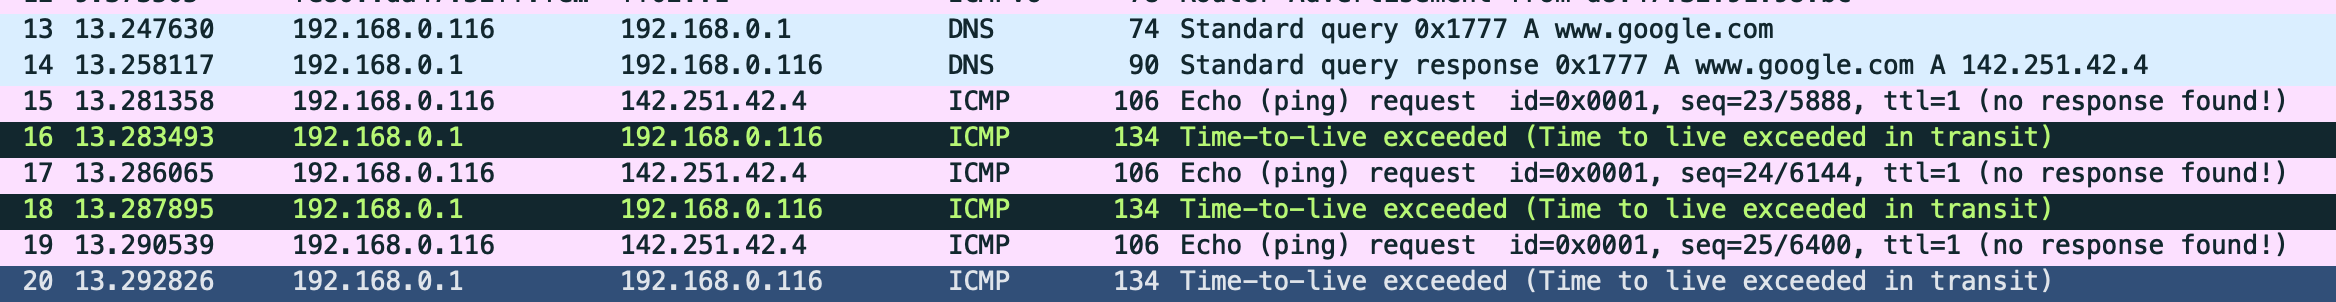
\includegraphics[width=1\linewidth]{images/image.png}
    \item Mac/Linux \texttt{traceroute} uses \textbf{UDP probes to high ports} by default.
    \\
    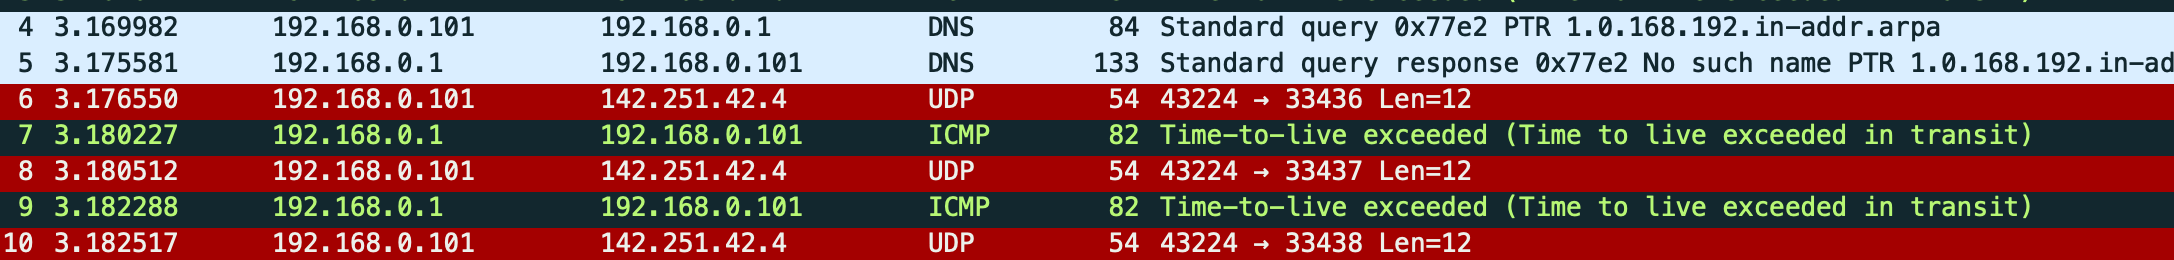
\includegraphics[width=1\linewidth]{images/image copy.png}
\end{itemize}

\textbf{Q2. Some hops in your traceroute output may show ``* * *''. Provide at least two reasons why a router might not reply.}

\textbf{Answer:}
\\  
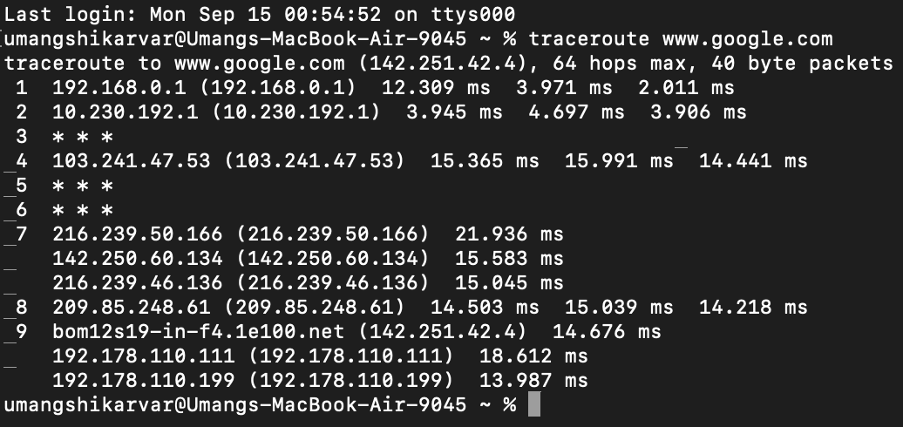
\includegraphics[width=1\linewidth]{images/Picture 1.png}
Possible reasons include:
\begin{itemize}[leftmargin=*]
    \item ICMP replies are blocked or rate-limited.  
    \item Firewall or router policy disallows \texttt{Time Exceeded} messages.  
    \item Router is overloaded and does not prioritize ICMP responses.
\end{itemize}

\textbf{Q3. In Linux traceroute, which field in the probe packets changes between successive probes sent to the destination?}

\textbf{Answer:}  In Mac/Linux traceroute, the \textbf{UDP destination port field} changes between successive probes.  
\\
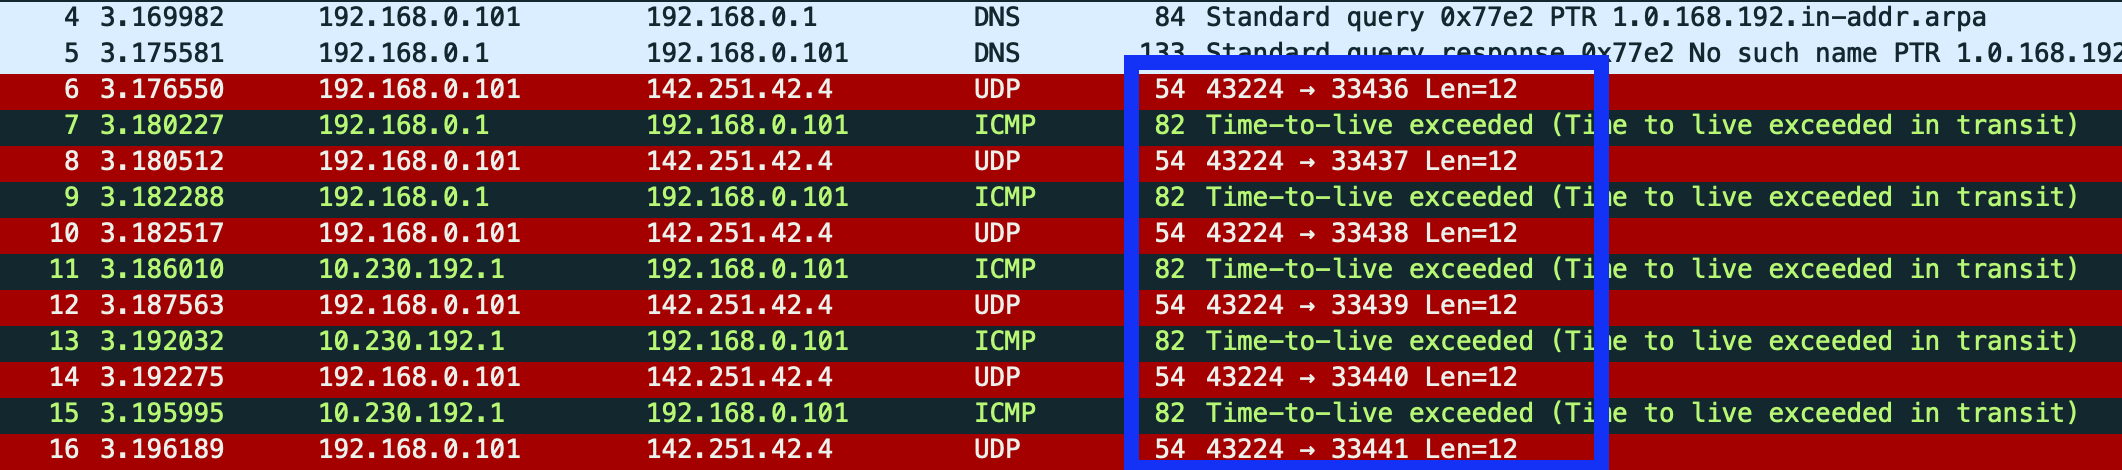
\includegraphics[width=1\linewidth]{images/image copy 2.png}

\textbf{Q4. At the final hop, how is the response different compared to the intermediate hop?}

\textbf{Answer:}  
\begin{itemize}[leftmargin=*]
    \item \textbf{Intermediate hops:} Send ICMP \texttt{Time-to-live exceeded}.
    \begin{itemize}
        \item Mac/Linux (UDP probes)
        \\
        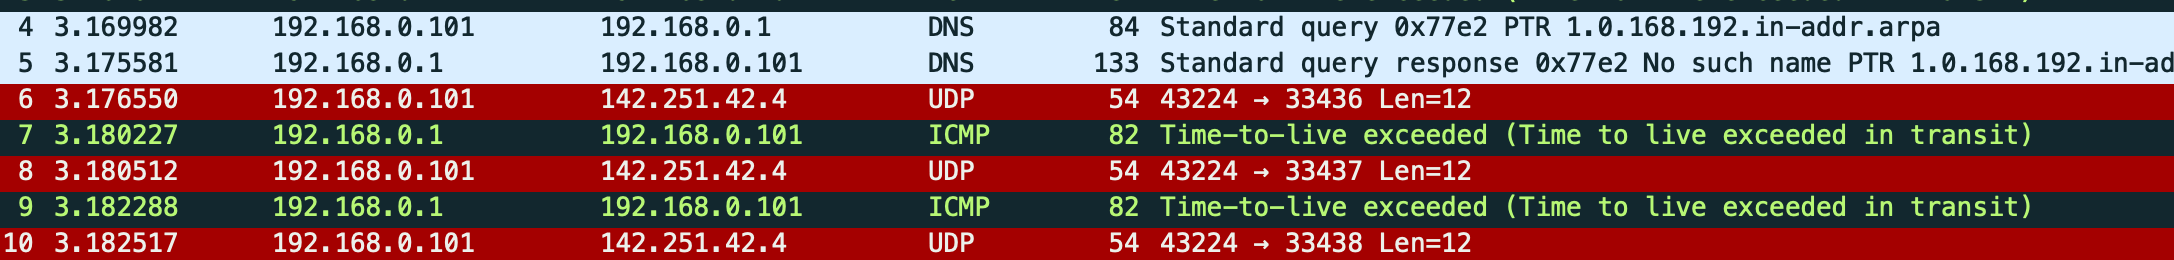
\includegraphics[width=1\linewidth]{images/image copy.png}
        \\
        \item On Windows (ICMP Echo probes)
        \\
        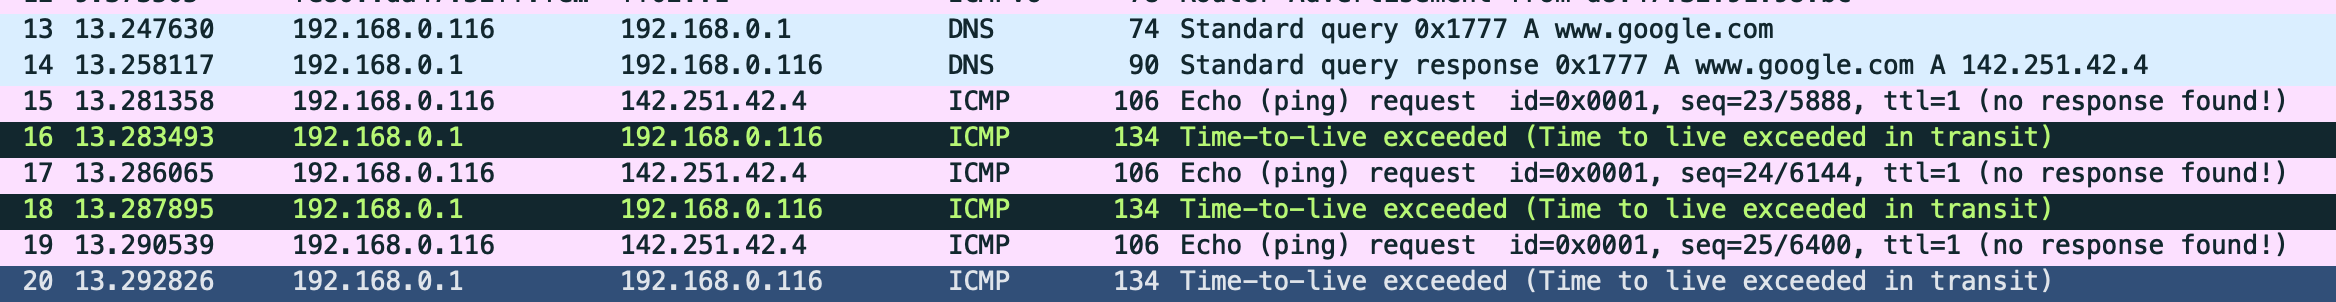
\includegraphics[width=1\linewidth]{images/image.png}
    \end{itemize}
    \item \textbf{Final hop:}  
    \begin{itemize}
        \item On Mac/Linux (UDP probes): ICMP \texttt{Destination Unreachable (Port Unreachable)}.
        \\
        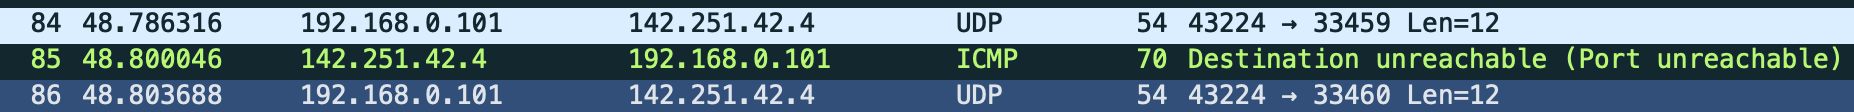
\includegraphics[width=1\linewidth]{images/image copy 3.png}
        \\
        \item On Windows (ICMP Echo probes): ICMP \texttt{Echo Reply}.
        \\
        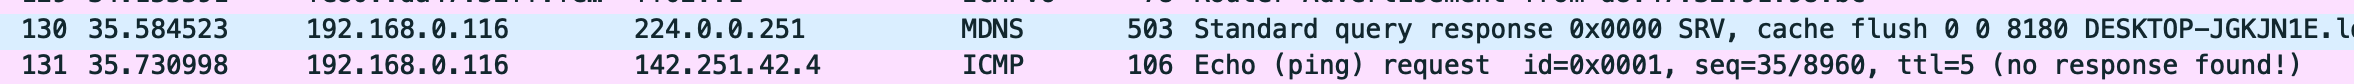
\includegraphics[width=1\linewidth]{images/image copy 4.png}
    \end{itemize}
\end{itemize}

\textbf{Q5. Suppose a firewall blocks UDP traffic but allows ICMP — how would this affect the results of Mac/Linux traceroute vs. Windows tracert?}

\textbf{Answer:}  
\begin{itemize}[leftmargin=*]
    \item \textbf{Mac/Linux (UDP-based):} Traceroute would fail because probes would never reach the destination (UDP blocked). Output would mostly show ``* * *''.  
    \item \textbf{Windows (ICMP-based):} Would still work normally, since probes are ICMP Echo Requests and replies would come back.  
\end{itemize}

\end{document}